\documentclass[12pt]{article}
\usepackage{hyperref}
\usepackage[warn]{mathtext}
\usepackage[T2A]{fontenc}
\usepackage[utf8]{inputenc}
\usepackage[russian]{babel}
\usepackage{cite}
\usepackage{amsfonts}
\usepackage{lineno}
\usepackage{subfig}
\usepackage{graphicx}
\usepackage{xcolor}
\usepackage{bm}
\usepackage{graphicx}
\usepackage{amssymb}
\usepackage{hyperref}
\usepackage[left=2cm,right=2cm,top=2cm,bottom=2cm]{geometry}

\DeclareGraphicsExtensions{.png,.jpg}
\date{14 сентября 2021 г.}
\author{Карцев Вадим}
\title{Лабораторная работа 2.1

Опыт Франка-Герца}

\begin{document}

\maketitle

\textbf{Цель работы:} измерение энергии первого уровня атомов гелия в динамическом и статическом режимах.

\textbf{В работе используются:} серийная лампа ионизационного манометра ЛМ-2, стабилизированный источник питания
Б7-4, микроамперметр, вольтметр, осцилограф C1-83.

\section{Теоретическая справка}
  Опыт Франка-Герца доказывает существование дискретных уровней энергии атома.

  В опыте используется трехэлектродная лампа, наполненная разреженным
  одноатомным газом.

  \begin {figure}[h!]
    \begin{minipage}[h]{0.49\linewidth}
        \center{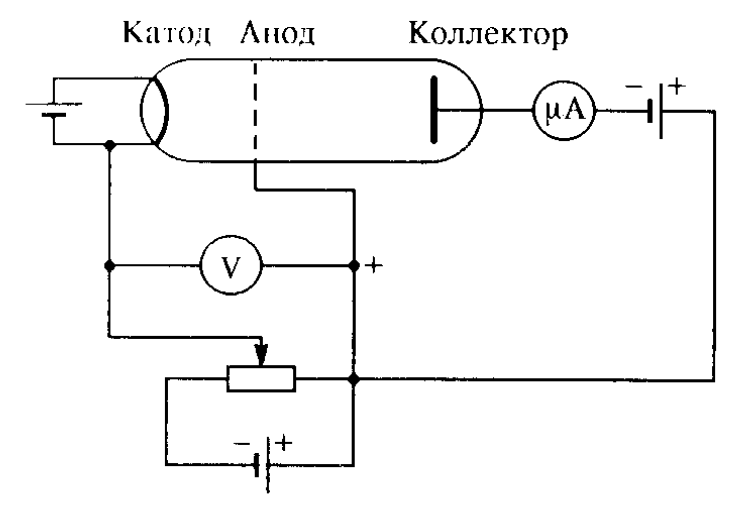
\includegraphics[width = 9cm]{ustanovka.png}}\\
        Рис 1. Схема установки
    \end{minipage}
    \begin{minipage}[h]{0.49\linewidth}
        \center{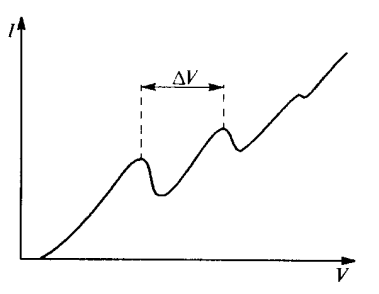
\includegraphics[width = 7cm]{scheme_plot.png}}\\
        Рис 2. Схематическая зависимость тока на коллекторе от разницы потенциалов между анодом и катодом
    \end{minipage}
    \label {fig:image1}
  \end {figure}

  Увеличивая разницу потенциалов между анодом и катодом мы увеличиваем энергия электронов.
  Пока энергии недостаточно для перевода атомов в возбужденное состояние, соударения будут практически
  упругими, т.к. масса электронов мала по сравнению с массой атомов. При дальнейшем увеличении энергии
  электронов начинает хватать для возбуждения или ионизации атомов газа и часть электронов теряет свою энергию
  при соударениях. Таким электронам не хватает энергии преодолеть задерживающее напряжение между анодом и
  коллектором и наблюдается резкое падение тока на последнем.

\section{Получение вольт-амперной характеристики $I_к = f(V_a)$ на экране осцилографа C1-83}

  Рассмотрим полученные осциллограммы

  \begin {figure}[h!]
    \begin{minipage}[h]{0.33\linewidth}
        \center{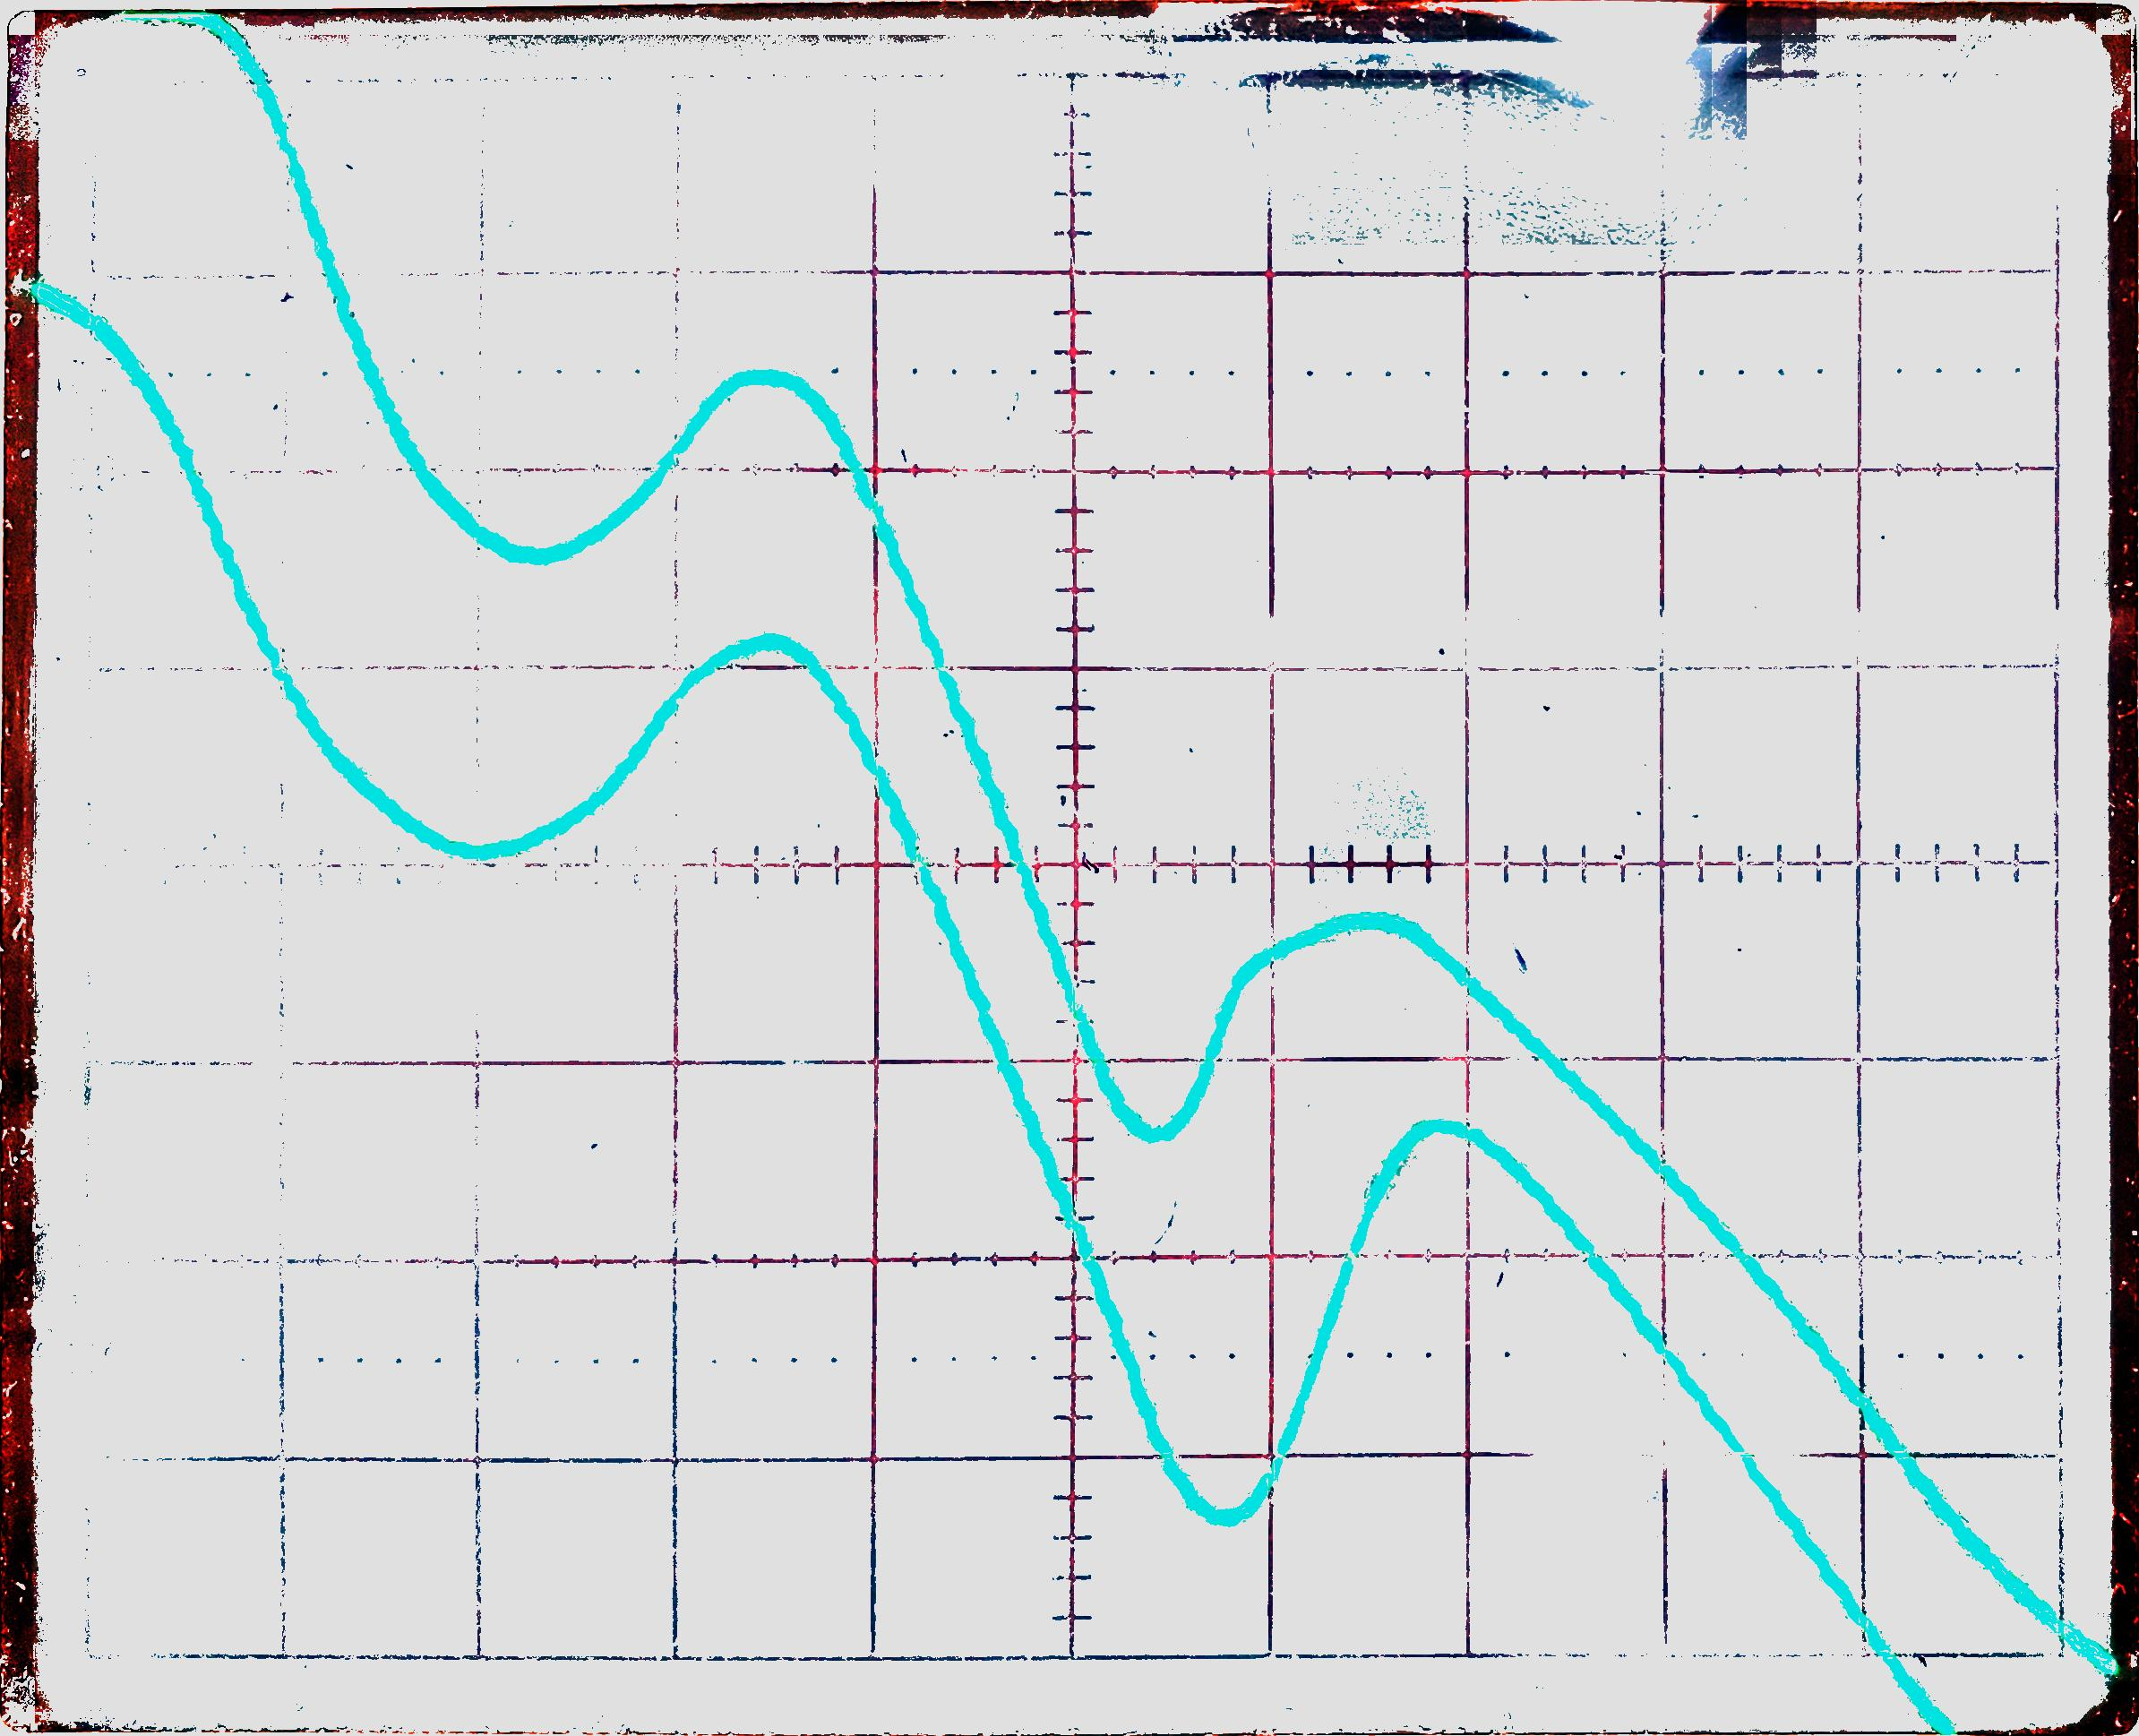
\includegraphics[width = 5.8cm]{oscillogram4V.jpg}}\\
        Рис 3. $V_2 = 4 В$
    \end{minipage}
    \begin{minipage}[h]{0.33\linewidth}
        \center{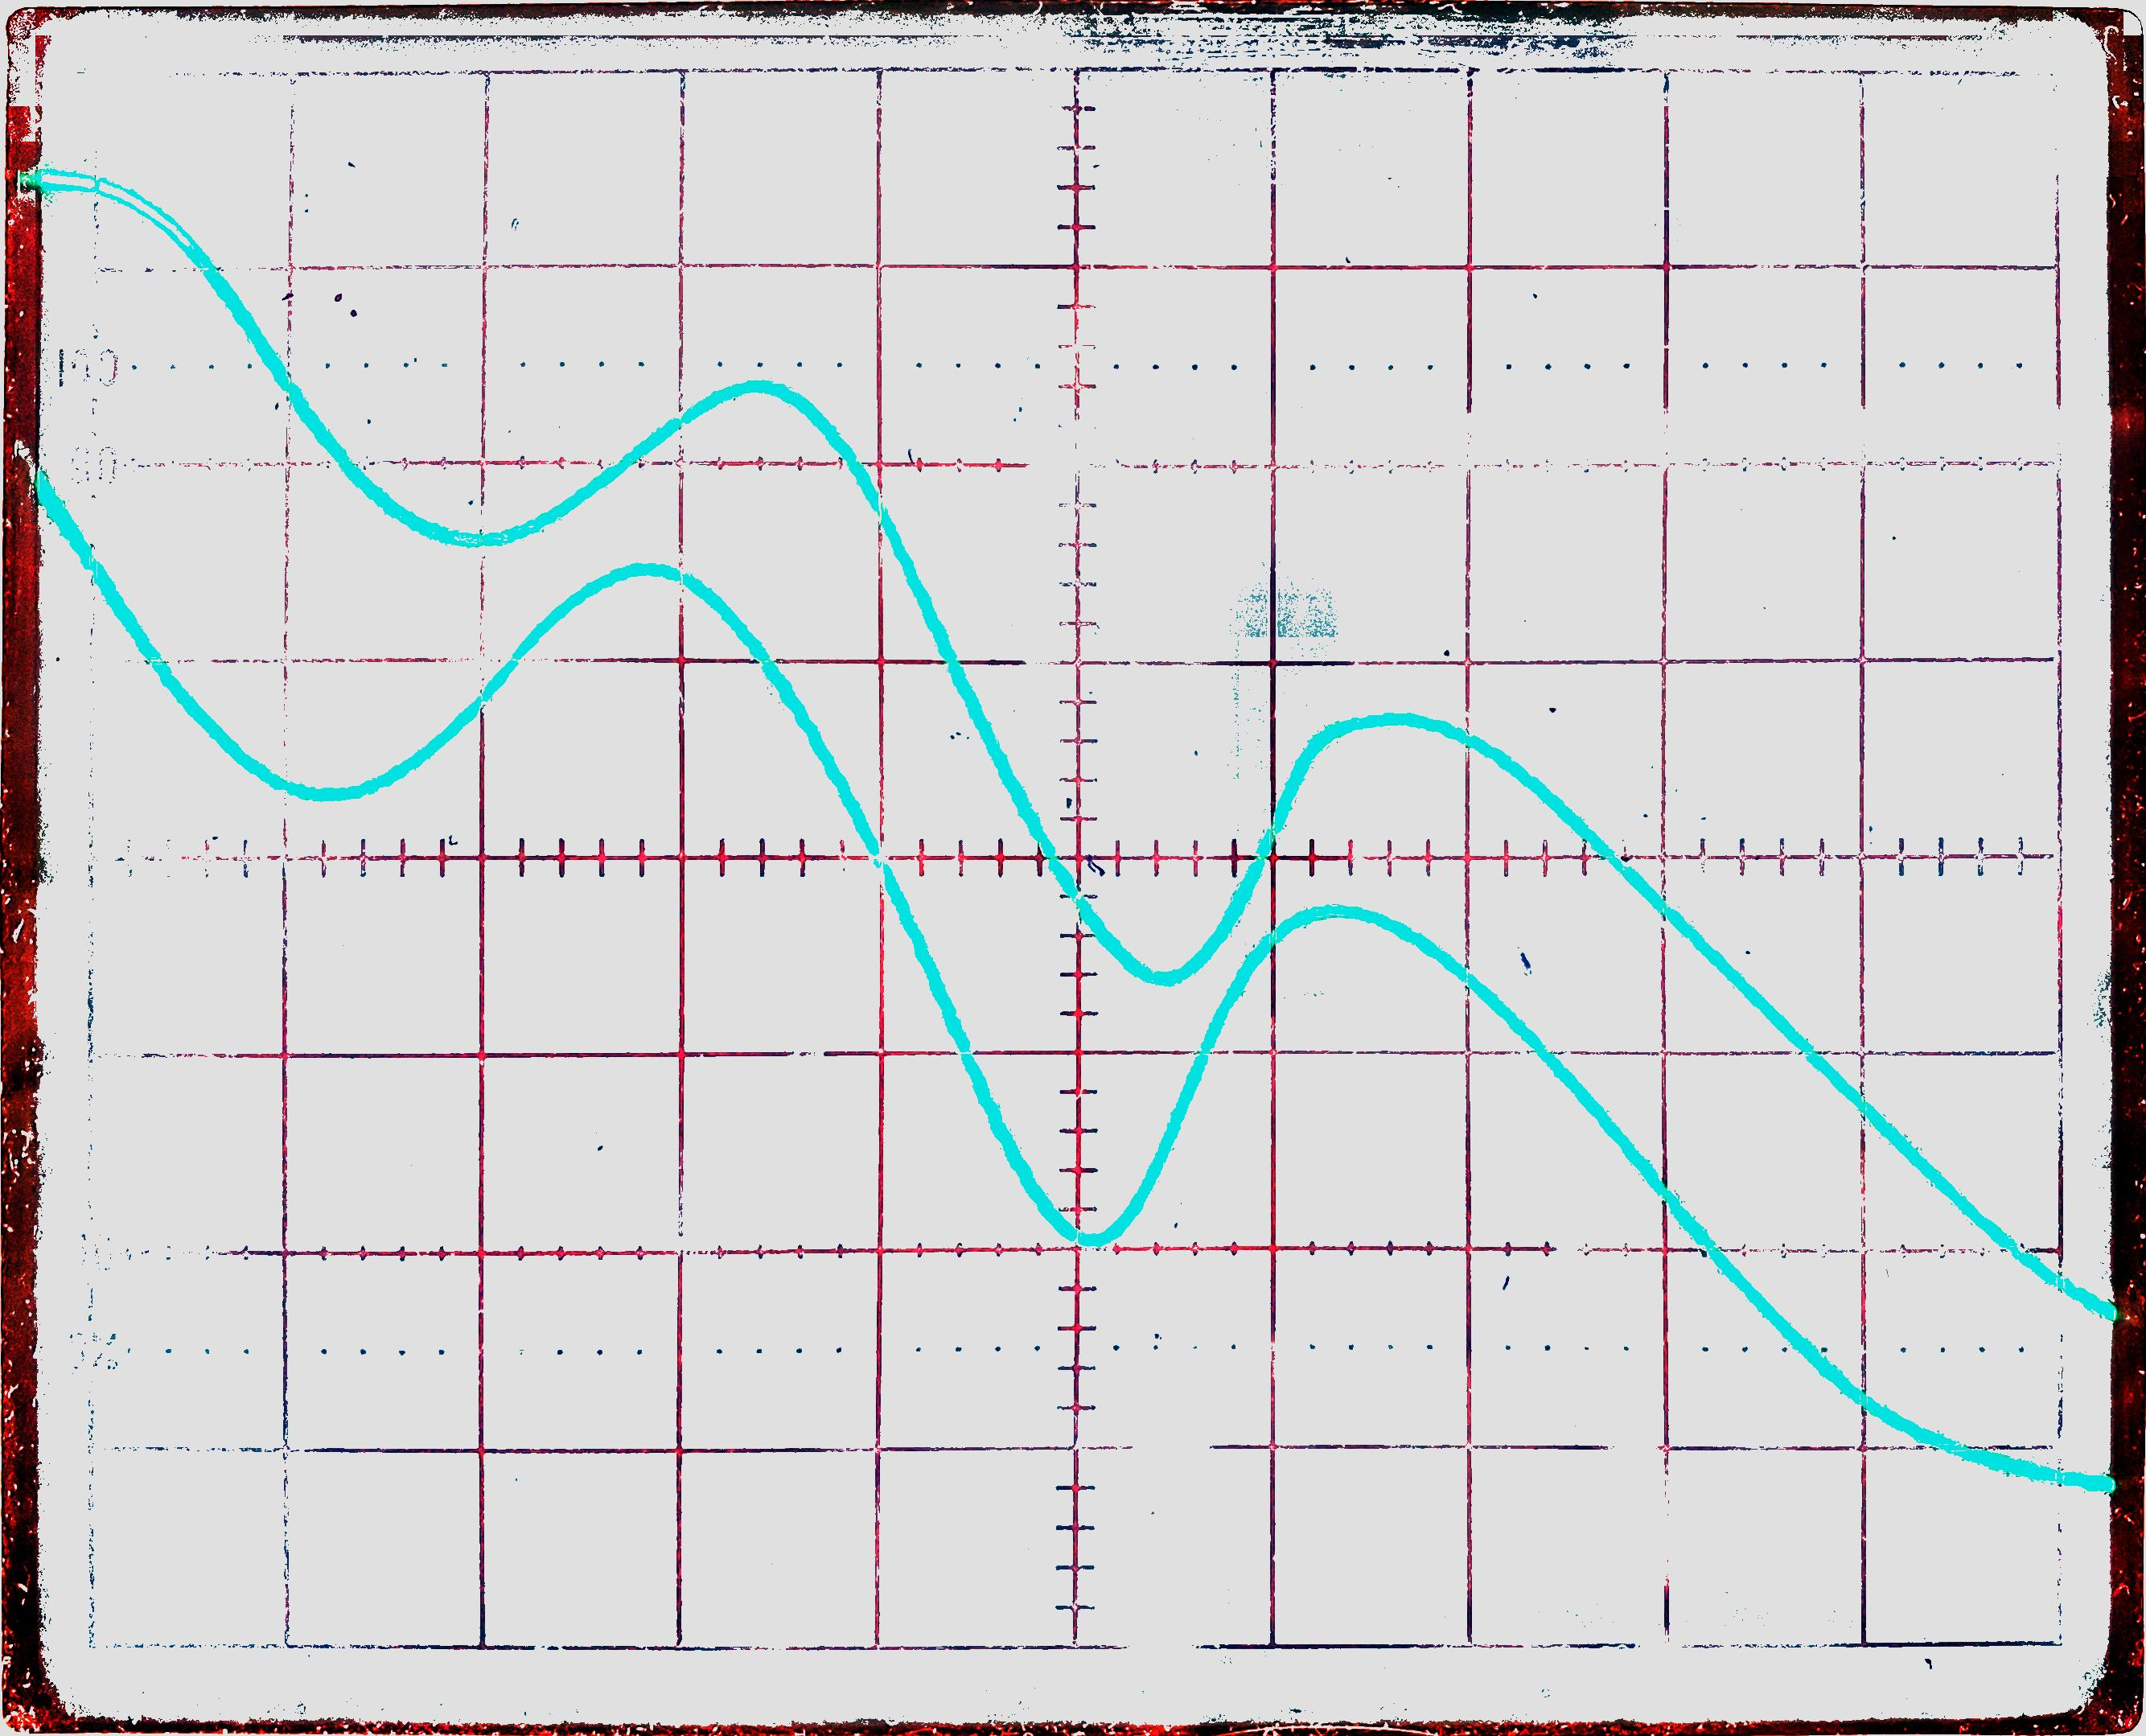
\includegraphics[width = 5.8cm]{oscillogram6V.jpg}}\\
        Рис 4. $V_2 = 6 В$
    \end{minipage}
    \begin{minipage}[h]{0.33\linewidth}
        \center{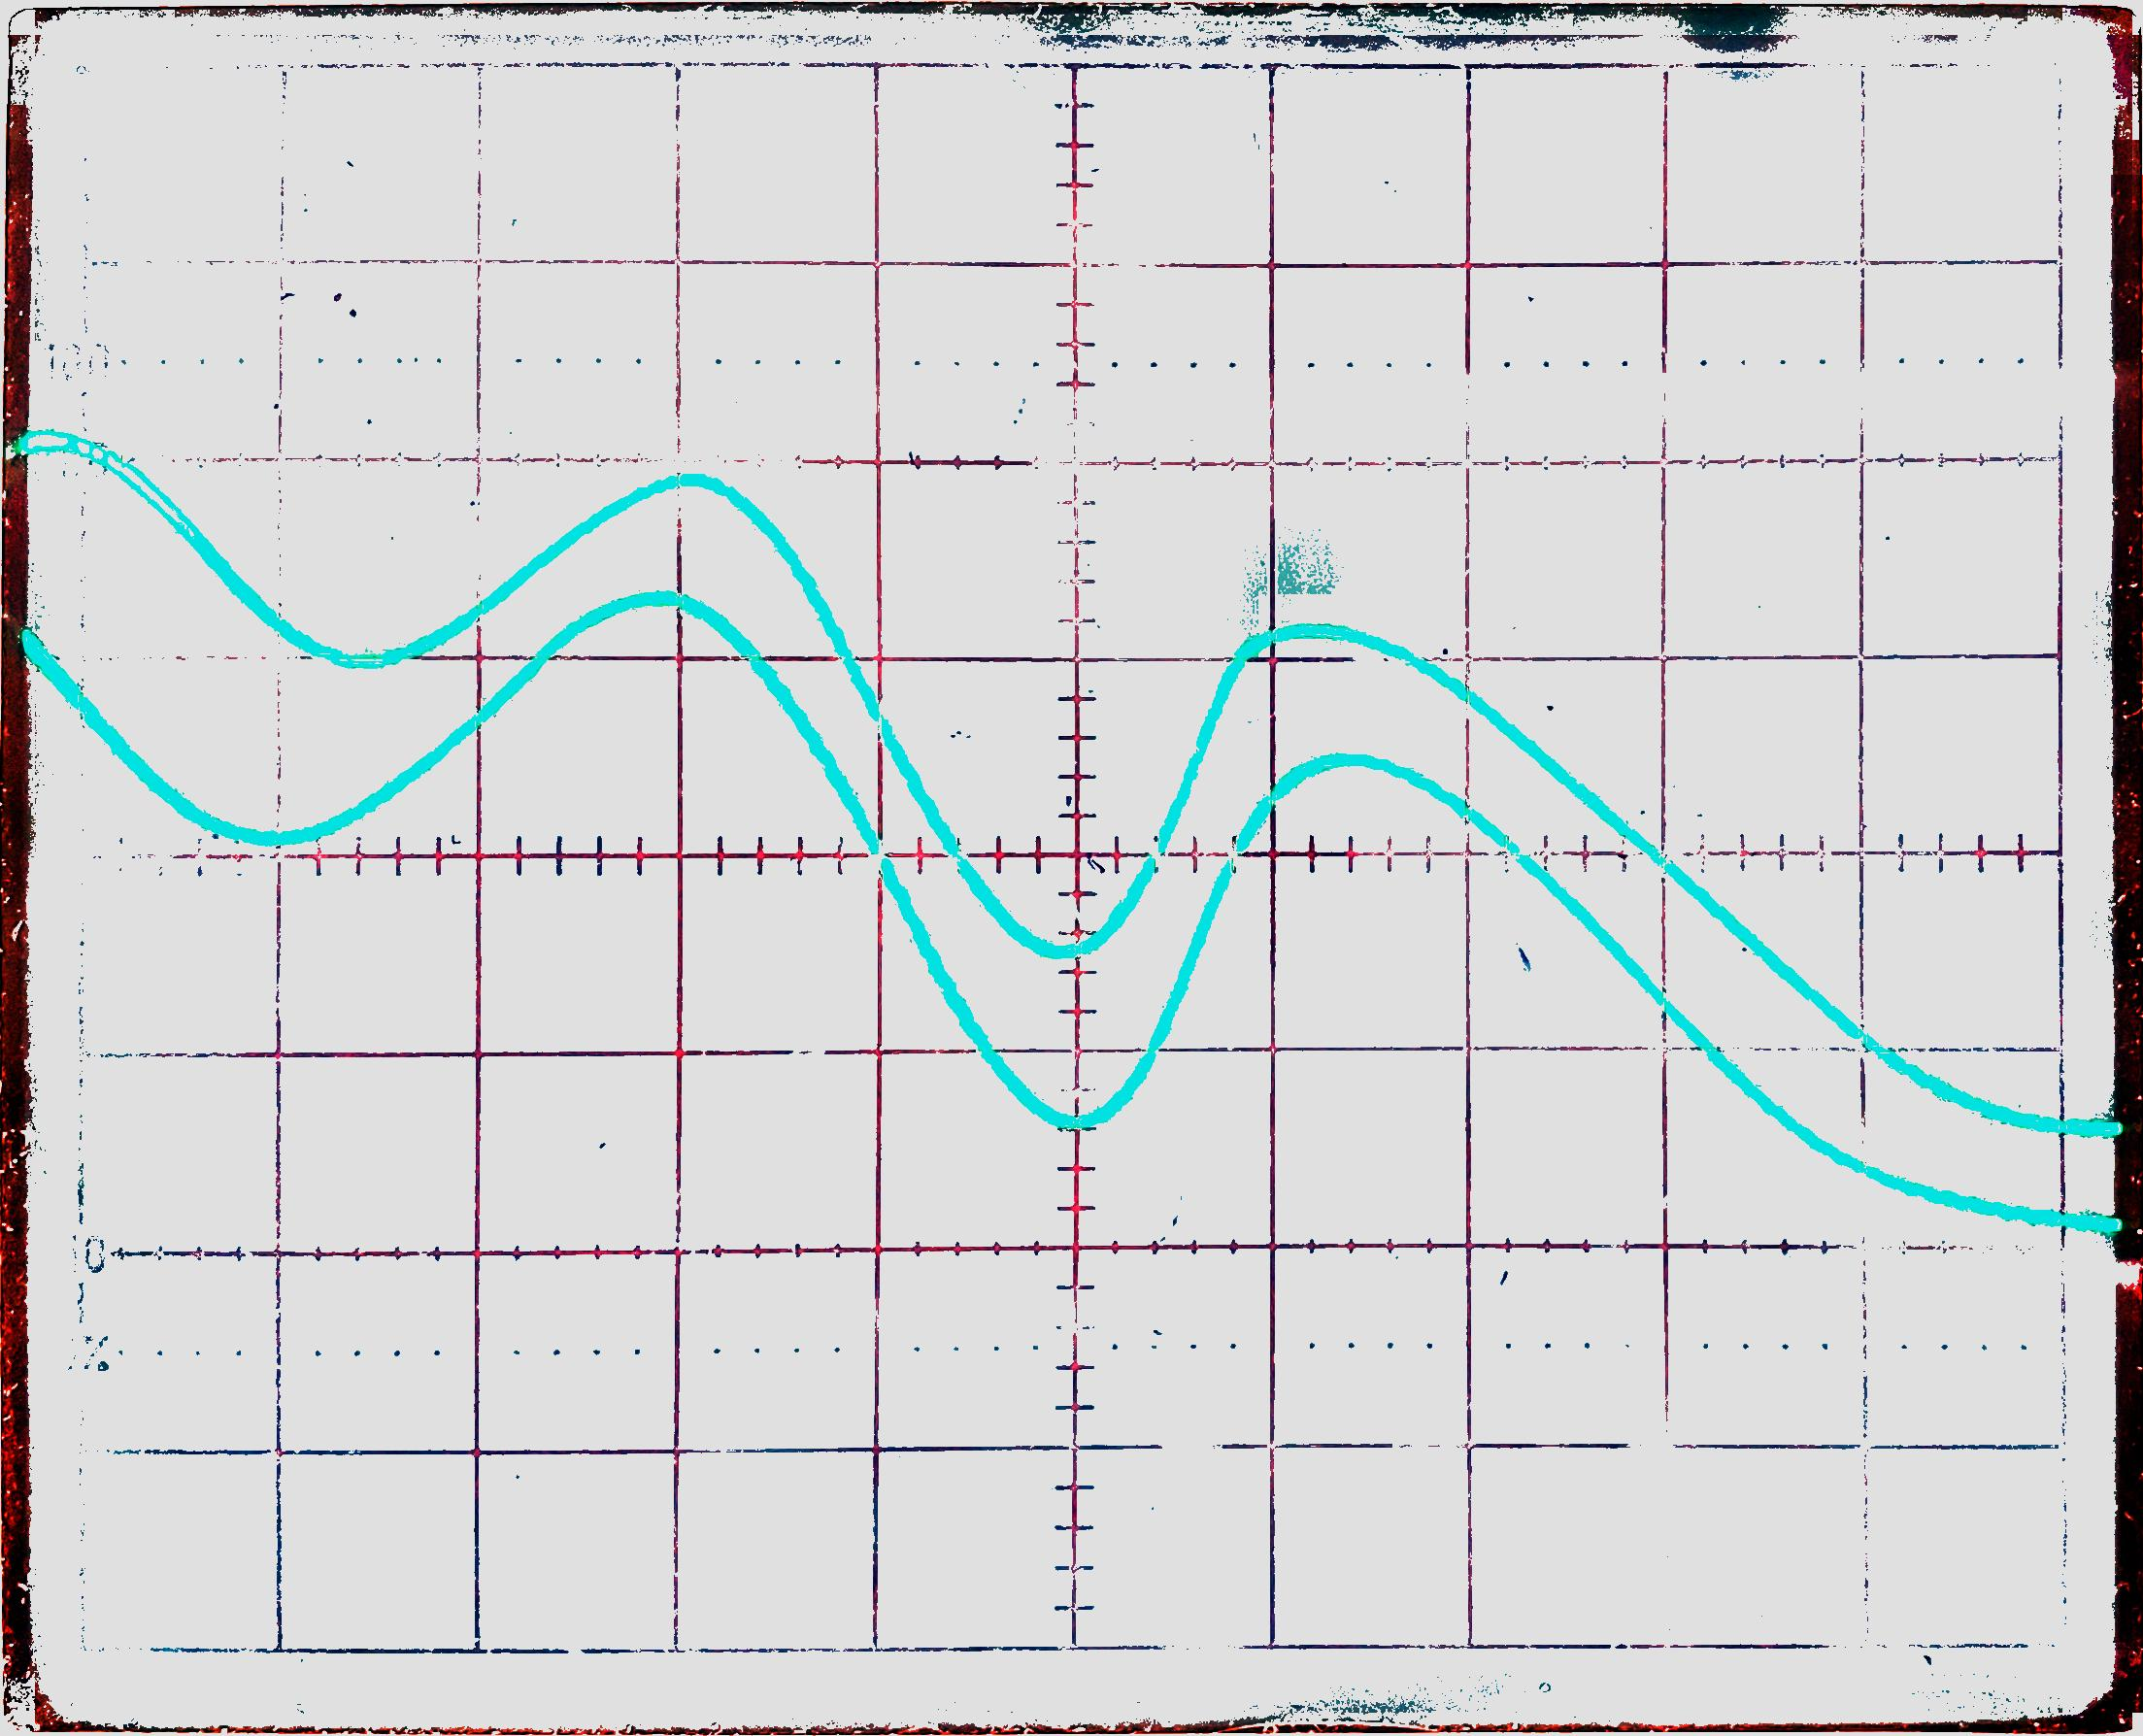
\includegraphics[width = 5.8cm]{oscillogram8V.jpg}}\\
        Рис 5. $V_2 = 8 В$
    \end{minipage}
    \label {fig:image1}
  \end {figure}

  Очевидно, на оцсиллограммах видны прямой и обратный ход. В первом случае напряжение повышается и видно, что ток
  на коллекторе растет с падениями, а во втором случае ток понижается со скачками. Все измерения на осцилографе
  проводились с разверткой $X = 5 В/дел$. Измерим расстояния между максимумами и минимумами в вольтах.

  \begin{figure}[h!]
    \center{Табл 1. Зависимость энергии возбуждения от напряжения торможения}
    \center{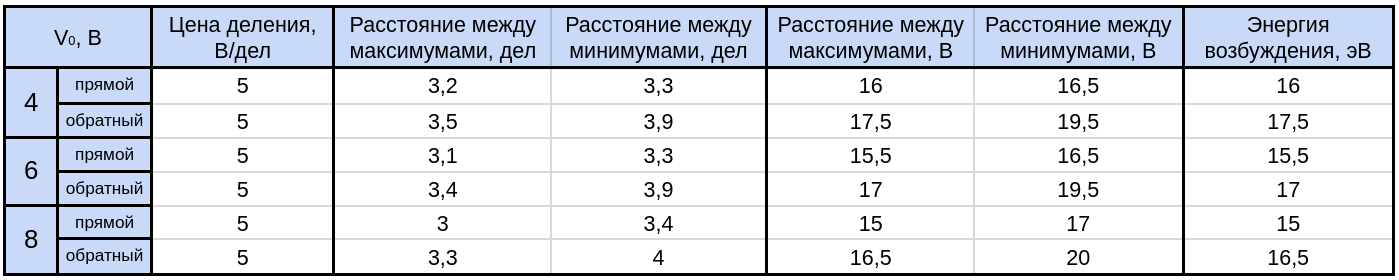
\includegraphics[width = 17.5cm]{table1.png}}
  \end{figure}

  Как видно из таблицы, энергия возбуждения атома гелия будет $E_{возб} = (16.25 \pm 0.94) эВ$, а относительная
  погрешность ее измерения $\varepsilon = 5.76\%$

  \newpage

\section{Получение вольт-амперной характеристики $I_к = f(V_a)$ в статическом режиме измерений}

\begin {figure}[h!]
  \begin{minipage}[h]{0.49\linewidth}
      Табл 2.
      \center{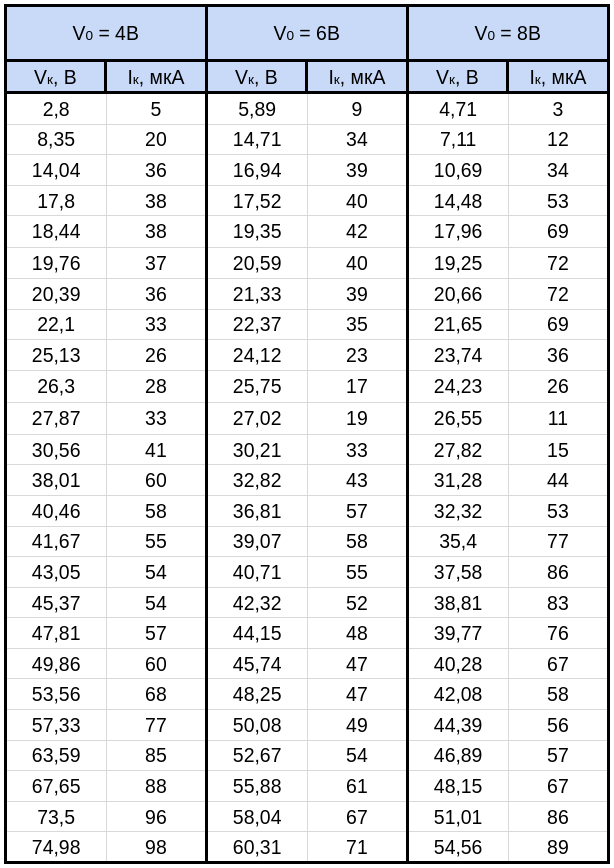
\includegraphics[width = 9cm]{table2.png}}\\
  \end{minipage}
  \begin{minipage}[h]{0.49\linewidth}
      \center{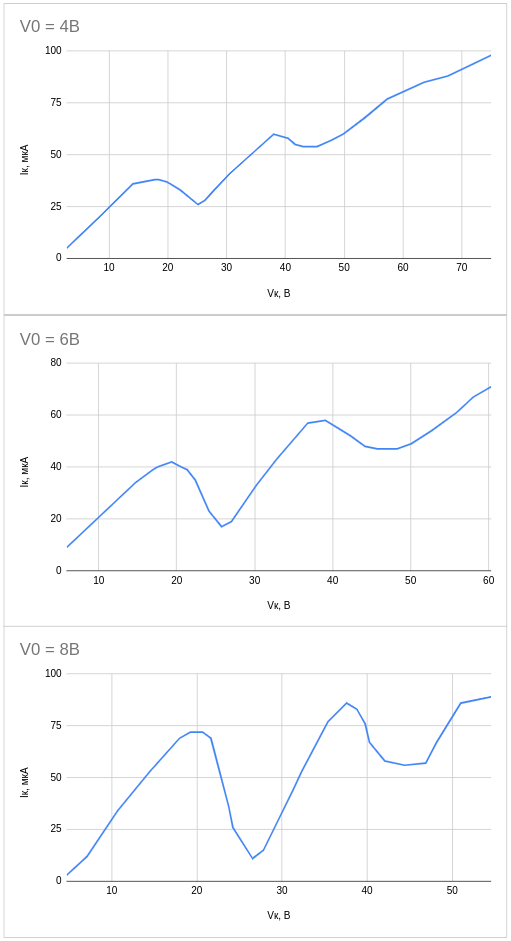
\includegraphics[width = 7cm]{plots.png}}\\
      Рис 6.
  \end{minipage}
  \label {fig:image1}
\end {figure}


\end{document}
